\documentclass[12pt]{article}
\usepackage{amsfonts, amsmath}
\usepackage{amssymb, geometry}
\usepackage{scalefnt}
\usepackage{setspace}
\usepackage{color,hyperref}
%\usepackage{epsfig,subfigure,morefloats}
\usepackage{natbib}
\usepackage{dsfont}
\usepackage{color,hyperref}
\usepackage{epstopdf}
\usepackage{amsthm}
\usepackage{amssymb}
%\usepackage{subcaption}
\usepackage{graphicx}
\usepackage{booktabs,siunitx}
\usepackage{bm}
\usepackage[section]{placeins}
%\usepackage{hypcap}
\usepackage{afterpage}


\setcounter{MaxMatrixCols}{10}

\providecommand{\u}[1]{\protect\rule{.1in}{.1in}}
\providecommand{\u}[1]{\protect\rule{.1in}{.1in}}
\newtheorem{theorem}{Theorem}
\newtheorem{acknowledgement}[theorem]{Acknowledgement}
%\newtheorem{algorithm}[theorem]{Algorithm}
\newtheorem{axiom}[theorem]{Axiom}
\newtheorem{case}[theorem]{Case}
\newtheorem{claim}{Claim}
\newtheorem{conclusion}[theorem]{Conclusion}
\newtheorem{condition}[theorem]{Condition}
\newtheorem{conjecture}{Conjecture}
\newtheorem{corollary}{Corollary}
\newtheorem{criterion}[theorem]{Criterion}
\newtheorem{definition}{Definition}
\theoremstyle{definition}
\newtheorem{example}{Example}
\newtheorem{exercise}{Exercise}
\newtheorem{lemma}{Lemma}
\newtheorem{notation}[theorem]{Notation}
\newtheorem{problem}[theorem]{Problem}
\newtheorem{proposition}{Proposition}
\newtheorem{remark}{Remark}
\newtheorem{solution}[theorem]{Solution}
\newtheorem{summary}[theorem]{Summary}
\geometry{left=1in,right=1in,top=1in,bottom=1in}
%\newenvironment{proof}[1][Proof]{\noindent\textbf{#1.} }{\ \rule{0.5em}{0.5em}}
%\hypersetup{pdftex,colorlinks=true,allcolors=black,citecolor=black}

\usepackage{floatrow}
\usepackage{algorithm}
\usepackage{algpseudocode}
\usepackage{float}
\usepackage{indentfirst}

\algnewcommand\algorithmicforeach{\textbf{for each}}
\algdef{S}[FOR]{ForEach}[1]{\algorithmicforeach\ #1\ \algorithmicdo}

\DeclareMathOperator*{\argmax}{arg\,max}
\DeclareMathOperator*{\argmin}{arg\,min}

%\graphicspath{{./Simulation_Graphs/}}

\usepackage{listings}
\usepackage{subcaption} 
\usepackage[toc,page]{appendix}
%\usepackage[extendedchars]{grffile}

\usepackage{mathpazo} % math & rm
\linespread{1.05}        % Palatino needs more leading (space between lines)
\usepackage[scaled]{helvet} % ss
\usepackage{courier} % tt
\normalfont
\usepackage[T1]{fontenc}

%% Math commands
\newcommand{\e}{\epsilon}
%\newcommand{\d}{\delta}
\newcommand{\D}{\Delta}
\newcommand{\R}{\mathbb{R}}
\newcommand{\Z}{\mathbb{Z}}
\usepackage{mathtools}
\DeclarePairedDelimiterX{\inp}[2]{\langle}{\rangle}{#1, #2}
\newcommand{\norm}[1]{\left\lVert#1\right\rVert}
\newcommand*{\vertbar}{\rule[-1ex]{0.5pt}{2.5ex}}
\newcommand*{\horzbar}{\rule[.5ex]{2.5ex}{0.5pt}}
\usepackage{mathrsfs}


\title{Matrix Methods in Machine Learning \\ Lecture Notes}
\author{Rebekah Dix}
\begin{document}
\maketitle
\tableofcontents
\newpage 

\section{Elements of Machine Learning}
\begin{enumerate}
	\item Collect data
	\item Preprocessing: changing data to simplify subsequent operations without losing relevant information.
	\item Feature extraction: reduce raw data by extracting features or properties relevant to the model.
	\item Generate training samples: a large collection of examples we can use to learn the model.
	\item Loss function: To learn the model, we choose a loss function (i.e. a measure of how well a model fits the data)
	\item Learn the model: Search over a collection of candidate models or model parameters to find one that minimizes the loss on training data.
	\item Characterize generalization error (the error of our predictions on new data that was not used for training).
\end{enumerate}

\section{Linear Algebra Review}

\subsection{Products}
Inner products:
\begin{equation}
	\inp{x}{w} = \sum_{j=1}^p w_j x_j = x^T w = w^T x
\end{equation}
Thus this inner product is a weighted sum of the elements of $x$.

Matrix-vector multiplication:
\begin{equation}
	Xw = 
	\begin{bmatrix}
	\horzbar x_1^T \horzbar \\
	\horzbar x_2^T \horzbar \\
	\vdots \\
	\horzbar x_n^T \horzbar
	\end{bmatrix}
	w
	=
	\begin{bmatrix}
	x_1^T w \\
	x_2^T w \\
	\vdots \\
	x_n^T w \\
	\end{bmatrix}
\end{equation}

Matrix-matrix multiplication:

\begin{example}
Let $X \in \R^{n \times p}$, $n$ movies, $p$ people. $T \in \R^{n \times r}$, and $W \in \R^{r \times p}$. We can think of $T$ as the taste profiles of $r$ representative customers and $W$ as the weights on each representative profile (there will be one set of weights for each customer). Suppose we have two representative taste profiles (i.e. an action lover and a romance lover). Then $w$ will be a $2$-vector containing the weights of on the two representative taste profiles. Then $Tw$ is the expected preferences of a customer who weights the representative taste profiles of $T$ with the weights given in $w$. 
\end{example}

Now we can think about the full matrix product $X = TW$
\begin{equation}
	X = TW \implies X_{ij} = \inp{i\text{th row of T}}{j\text{th column of W}}
\end{equation}

\begin{itemize}
	\item The $j$th column of $X$ is a weighted sum of the columns of $T$, where the $j$th column of $W$ tells us the weights.
	\begin{equation}
		x_j = T w_j 
	\end{equation}
	That is, the tastes (preferences) of the $j$th customer.
	\item The $i$th row of $X$ is $x_i^T = t_i^T W$ where $t_i^T$ is the $i$th row of $T$. This gives us how much each customer likes movie $i$. 
\end{itemize}

Inner product representation:
\begin{equation}
	TW = 
	\begin{bmatrix}
	\horzbar t_1^T \horzbar \\
	\horzbar t_2^T \horzbar \\
	\vdots \\
	\horzbar t_n^T \horzbar	
	\end{bmatrix}
	\begin{bmatrix}
	\vertbar & \vertbar & & \vertbar\\
	w_1 & w_2 & \ldots & w_p \\
	\vertbar & \vertbar & & \vertbar\\	
	\end{bmatrix}
	=
	\begin{bmatrix}
	t_1^Tw_1 & t_1^Tw_2 & \hdots & t_1^Tw_p \\
	t_2^Tw_1 & \ddots & & \vdots\\
	\vdots & & \ddots & \vdots \\
	t_n^Tw_1 & & & t_n^Tw_p
	\end{bmatrix}
\end{equation}

Outer Product Representation:
\begin{equation}
	TW = 
	\begin{bmatrix}
	\vertbar & \vertbar & & \vertbar\\
	T_1 & T_2 & \ldots & T_r \\
	\vertbar & \vertbar & & \vertbar\\	
	\end{bmatrix}
	\begin{bmatrix}
	\horzbar w_1^T \horzbar \\
	\horzbar w_2^T \horzbar \\
	\vdots \\
	\horzbar w_r^T \horzbar	
	\end{bmatrix}
	= \sum_{k=1}^r T_k w_k^T
\end{equation}
(the sum of rank $1$ matrices. $TW$ has rank $r$ if and only if the columns of $T$ are rows of $W$ are linearly independent). In this representation, we can think about $T_k$ as the $k$th representative taste profile and $w^T_k$ as the $k$th row of $W$, or the affinity of each customer with the $k$th representative profile. 

\subsection{Linear Independence}
\begin{definition}(Linear Independence)
Vectors $v_1, v_2, \ldots, v_n \in \R^p$ are linearly independent vectors if and only if
\begin{equation}
	\sum_{j=1}^n \alpha_j v_j = 0 \iff \alpha_j = 0, j=1,\ldots,n
\end{equation}	
\end{definition}

\begin{definition}(Matrix rank)
The rank of a matrix is the maximum number of linearly independent columns. The rank of a matrix is less than the smallest dimension of the matrix. 
\end{definition}


\section{Linear Systems and Vector Norms}

\begin{example}(Condition on $rank(A)$ for existence of exact solution)

Consider the linear system of equations $Ax = b$. This means that $b$ is a weighted sum of the columns of $A$. Suppose $A$ is full rank. Now consider the matrix $\begin{bmatrix} A & b\end{bmatrix}$. If the rank of $\begin{bmatrix} A & b\end{bmatrix}$ were \textit{greater} than the rank of $A$ (since the number of columns of the matrix increased by $1$ and $A$ is assumed full rank, this would imply the rank is $rank(A) + 1$), this would mean that $b$ could not be written as a linear combination of the columns of $A$, and that the system would not have an exact solution. Therefore, we must have that $rank (\begin{bmatrix} A & b\end{bmatrix}) = rank(A)$ in order for the system $Ax = b$ to have an exact solution. 

To see how the definition of linear independence applies here, observe that $Ax = b \implies Ax - b = 0$. Therefore
\begin{equation}
	\begin{bmatrix}
	A & b
	\end{bmatrix}
	\begin{bmatrix}
	x \\
	-1
	\end{bmatrix}
	=
	0
\end{equation}
Thus, if $Ax = b$ has an exact solution, then $\begin{bmatrix} A & b\end{bmatrix}$ does not have linearly independent columns. 
\end{example}

\begin{example}(Condition on $rank(A)$ for more than one exact solution)

If the system of linear equations $Ax = b$ has more than one exact solution, then there is at least one non zero vector $w$ for which $x+w$ is also a solution. That is, $A(x + w) = b$. If $x$ is an exact solution, then $Ax = b$. This implies $Aw = 0$. Therefore, the columns of $A$ are linearly dependent. Thus, if $rank(A) < dim(x)$, then there will be more than one exact solution. 
\end{example}

\begin{example}(Apply the above conditions)
Let
\begin{equation}
	A = 
	\begin{bmatrix}
	1 & -2 \\
	-1 & 2 \\
	-2 & 4
	\end{bmatrix},
	\quad
	b = 
	\begin{bmatrix}
	2 \\ -2 \\ -4
	\end{bmatrix}
\end{equation}
We want to solve $Ax = b$. 
\begin{itemize}
	\item This system has an exact solution, since $rank(A) = rank(\begin{bmatrix} A & b\end{bmatrix})$. This follows since the columns of $A$ are linearly dependent, so it has rank $1$, and $b$ is a multiple of the columns of $A$, so the rank of $\begin{bmatrix} A & b\end{bmatrix}$ is also 1. 
	\item Note that $1 = rank(A) < dim(x) = 2$. Therefore this system does not have a unique solution. 
\end{itemize}
\end{example}

\subsection{Vector Norms}

\begin{definition}(Vector Norm)
A vector norm is a function $\norm{\cdot}$ mapping from $\R^n \to \R$ with the following properties. 
\begin{enumerate}
	\item $\norm{x} \geq 0$ for all $x \in \R^n$.
	\item $\norm{x} = 0$ if and only if $x = 0$. 
	\item $\norm{\alpha x} = |\alpha|\norm{x}$ for all $\alpha \in \R$, $x \in \R^n$. 
	\item $\norm{x + y} \leq \norm{x} + \norm{y}$ for all $x, y \in \R^n$. 
\end{enumerate}
\end{definition}

Helpful fact: $\norm{x}_{q'} \leq \norm{x}_q$ if $1 \leq q \leq q' \leq \infty$. 

\begin{figure}[H]
	\begin{center}
		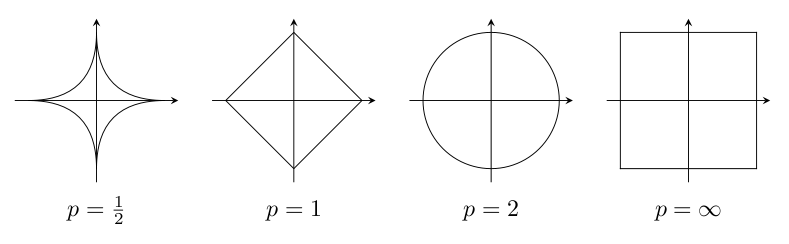
\includegraphics[scale=.5]{norm_ball.png}
	\end{center}
	\caption{The $l_p$ norm in $\R^2$}
\end{figure}

\section{Least Squares}
We are given:
\begin{enumerate}
	\item Vector of labels $y \in \R^n$ 
	\item Matrix of features $X \in \R^{n \times p}$
\end{enumerate}

We want to find:
\begin{enumerate}
	\item Vector of weights $w \in \R^p$
\end{enumerate}

Assumptions:
\begin{enumerate}
	\item $n \geq p$, and $rank(X) = p$. 
\end{enumerate}

If $y = Xw$, then we have a system of $n$ linear equations, where the $i$th equation is
\begin{equation}
	y_i = w_1 x_{i1} + w_2 x_{i2} + \cdots + w_p x_{ip} = \sum_{j=1}^p w_j x_{ij} = \inp{w}{x_{\cdot i}}
\end{equation}
where $x_{\cdot i}$ is the $i$th row of $X$. 

In general, $y \neq Xw$ for any $w$. We define a residual $r_i = y_i - \inp{w}{x_{\cdot i}}$. Our goal is then to find $w$
$\sum_{i=1}^n |r_i|^2$ (the sum of square residuals/errors). 

Why should we minimize the sum of square errors?
\begin{enumerate}
	\item Magnifies the effect of large errors
	\item Allows us to compute derivatives
	\item Simple geometric interpretation
	\item Coincides with modeling $y = Xw + \e$, where $\e $ is Gaussian noise
\end{enumerate}

\subsection{Geometric Approach}

We know $\hat r = y - X \hat w$ is orthogonal to the span of the columns of $X$. Thus $x_i^T \hat r = 0$, or $X^T \hat r = 0$. This implies $X^T (y - X \hat w) = 0$. Thus $\hat w$ is a solution to the linear system of equations
\begin{equation}
	X^T X \hat w = X^T y
\end{equation}

\begin{figure}[H]
	\begin{center}
		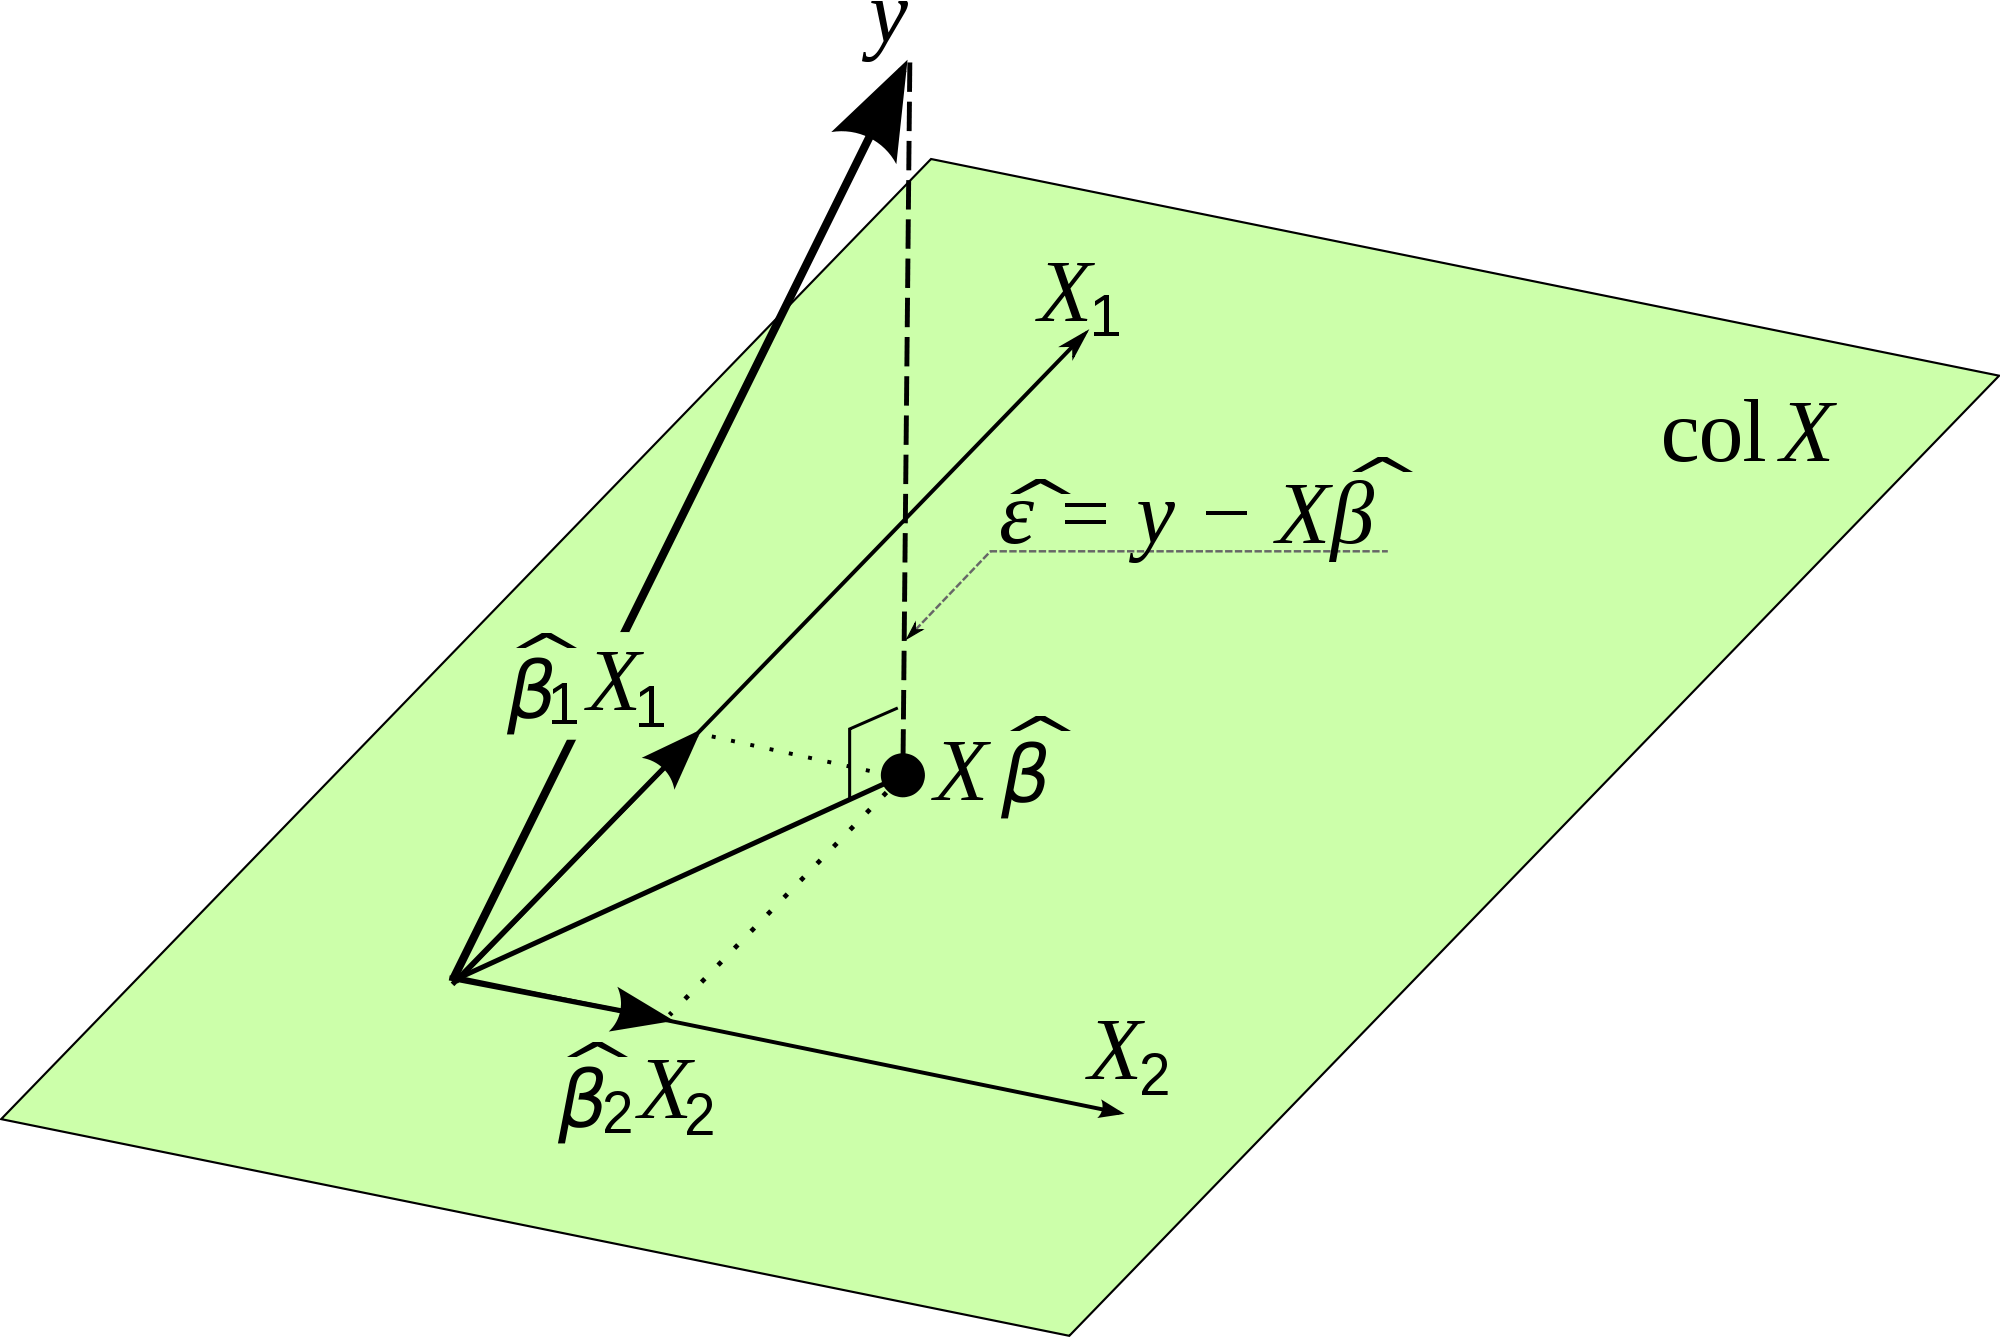
\includegraphics[scale=.1]{ls_geometry.png}
	\end{center}
	\caption{Geometry of LS in $\R^2$}
\end{figure}

Observations:
\begin{itemize}
	\item The question we're trying to answer: What is the point in $col(X)$ that has the shortest distance to $y$? In $\R^2$, what are the weights $\beta_1$ and $\beta_2$ such that $\beta_1 x_1 + \beta_2 x_2$ has the shortest distance to $y$?
	\item $col X$ is the space of all vectors that can be written as $\alpha x_1 + \beta x_2$ for some $\alpha, \beta \in \R$, that is the span of the columns of $X$. $y$ may not lie in this space. 
	\item The residual vector will form a right angle with $col X$, because any other angle would correspond to a longer distance. 
\end{itemize}

\subsection{Vector Calculus Approach}
\subsubsection{Review of Vector Calculus}
Let $w$ be a $p$-vector and let $f$ be a function of $w$ that maps $\R^p$ to $\R$. Then the gradient of $f$ with respect to $w$ is
\begin{equation}
	\nabla_w f(w) = \begin{pmatrix} \frac{\partial f(w)}{\partial w_1} \\ \vdots \\ \frac{\partial f(w)}{\partial w_p} \end{pmatrix}
\end{equation}

\begin{example}(Gradient of an Inner Product)
Let $f(w) = \inp{a}{w} = w^T a = \sum_{i=1}^n w_i a_i$. Then
\begin{equation}
	\nabla_w w^T a = \begin{pmatrix} a_1 \\ a_2 \\ \vdots \\ a_p \end{pmatrix} = a
\end{equation}
\end{example}

\begin{example}(Gradient of an Inner Product, Squared)
Let $f(w) = \norm{w}^2 = w^T w = w_1^2 + \cdots + w_p^2$. Then 
\begin{equation}
	\nabla_w w^T w = \begin{pmatrix} 2w_1 \\ 2w_2 \\ \vdots \\ 2w_p \end{pmatrix} = 2w
\end{equation}
(This is a special case of the Quadratic Form discussed below, where $w^TQw$, and $Q=I$)
\end{example}

\begin{example}(Gradient of a Quadratic Form)
Let $x \in \R^n$ and $f(x) = x^T Q x$, where $Q$ is symmetric (if $Q$ isn't symmetric we could replace $Q$ with $\frac{1}{2}(Q + Q^T)$).
Then
\begin{align*}
	f(x) &= x^T Q x \\
	&= \sum_{i=1}^n \sum_{j=1}^n x_i Q_{ij}x_j
\end{align*}
Therefore
\begin{equation}
	[\nabla_x f]_k = \frac{d f}{d x_k} = \begin{cases}
	2 Q_{kk} x_k & i=j=k \\
	Q_{kj} x_j & i =k, i \neq j \\
	Q_{ik} x_i & j = k, j \neq i
	\end{cases}
\end{equation}
Therefore
\begin{equation}
	\nabla_x f = (Q + Q^T) x 
\end{equation}
If $Q$ is symmetric, then this equals $2Qx$.
\end{example}

\subsubsection{Application to Least Squares}
Let $f(w) = \norm{y - Xw}_2^2$. Then the least squares problem is 
\begin{equation}
	\hat{w} = \argmin_w f(w)
\end{equation}
We can expand $f(w)$ as
\begin{align*}
	f(w) &= (y - Xw)^T(y - Xw) \\
	&= y^T y - y^T X w - w^T X^T y + w^T X^T X w \\
	&= y^T y - 2 w^T X^T y + w^T X^T X w
\end{align*}
Then
\begin{align*}
	\nabla_w f(w) = -2 X^T y + 2 X^T X w
\end{align*}
At an optimum we have that $\hat{w}$ solves $X^T y = X^T X w$. Then if $(X^T X)^{-1}$ exists, we have that
\begin{equation}
	\hat{w} = (X^T X)^{-1} X^T y
\end{equation}

\begin{theorem}(Sufficient Condition for Existence/Uniqueness of LS Solution)
If the columns of $X$ are linearly independent, then $X^T X$ is non-singular, and there exists a unique least squares solution $\hat{w} = (X^T X)^{-1} X^T y$.
\end{theorem}

\begin{proof}

\end{proof}

\subsection{Positive Definite Matrices}
\begin{definition}[Positive Definite, pd]
A matrix $Q$ ($n \times n$) is positive definite (written $Q \succ 0$) if $x^T Q x > 0$ for all $x \in \R^n$, $x \neq 0$. 
\end{definition}

\begin{definition}[Positive Semi-Definite, psd]
A matrix $Q$ ($n \times n$) is positive semi-definite (written $Q \succeq 0$) if $x^T Q x \geq 0$ for all $x \in \R^n$, $x \neq 0$. 
\end{definition}

Properties of Positive Definite matrices:
\begin{enumerate}
	\item If $P \succ 0$ and $Q \succ 0$, then $P+Q \succ 0$.
	\item If $P \succ 0$ and $\alpha > 0$, then $\alpha P \succ 0$.
	\item For any matrix $A$, $A^T A \succeq 0$ and $AA^T \succeq 0$. Further, if the columns of $A$ are linearly independent, then $A^T A \succ 0$.
	\item If $A \succ 0$, then $A^{-1}$ exists.
	\item Notation: $A \succ B$ means $A - B \succ 0$.
\end{enumerate}


\begin{example}
Let
\begin{equation}
	X = 
	\begin{pmatrix}
	1 & 1 \\
	1 & 1 \\
	1 & 1
	\end{pmatrix}
\end{equation}
Then 
\begin{equation}
	X^T X = 
	\begin{pmatrix}
	3 & 3 \\
	3 & 3
	\end{pmatrix}
\end{equation}
Consider the vector $a = \begin{pmatrix} 1 \\ -1 \end{pmatrix}$. Then $a^T X^T X a = 0$. Therefore $X^T X$ is not positive definite. 
\end{example}	

\subsection{Subspaces}
\begin{definition}(Subspace)
A set of points $S \subseteq \R^n$ is a subspace if
\begin{enumerate}
	\item $0 \in S$ ($S$ contains the origin)
	\item If $x,y \in S$, then $x + y \in S$
	\item If $x \in S$, $\alpha \in \R$, then $\alpha x \in S$.
\end{enumerate}
\end{definition}

\subsection{Least Squares with Orthonormal Basis for Subspace}
Suppose are given a training sample $\{x_i, y_i \}_{i=1}^n$, $x_i \in \R^p$ and $y\in \R$. If the columns of $X$ (the data matrix) are linearly dependent, then $X^TX$ is not invertible. It is then impossible to tell which features are significant predictors of $y$. 

Given $X = \begin{bmatrix} x_1 \ldots x_p \end{bmatrix}$, the following are options to represent the corresponding subspace spanned by the columns of $X$: 
\begin{enumerate}
	\item  Use $X$, but then $LS$ can be hard to interpret.
	\item Use an orthonormal basis for the subspace.
\end{enumerate}

\subsubsection{Orthogonal Matrices and Orthonormal Basis}

\begin{definition}(Orthonormal basis for $X$)
An orthonormal basis for the columns of $X$ is a collection of vectors $\{u_1, \ldots, u_r \}$ such that the span of the columns of $X$ equals the span of $\{u_1, \ldots, u_r \}$. That is, $span(\{x_1, \ldots, x_p\}) = span(\{u_1, \ldots, u_r \})$. Furthermore, 
\begin{equation}
	u_i^T u_j = 
	\begin{cases}
	0 & i\neq j \\
	1 & i = j
	\end{cases}
\end{equation}
That is, the $u$ vectors are orthogonal and have norm $1$. 
\end{definition}

Observations:
\begin{itemize}
	\item The rank $r$ of the subspace must satisfy $r \leq \min{(n,p)}$. $r$ is the number of linearly independent columns of $X$. 
	\item We can place the basis vectors into a basis matrix $U \in \R^{n \times r}$. 
\end{itemize}

\begin{claim}(Properties of orthogonal (basis) matrices)
Let $U \in \R^{n \times r}$ be an orthogonal (basis) matrix.   
\begin{enumerate}
	\item $U^T U = I$
	\item If $U$ and $V$ are both orthogonal, then $UV$ is also orthogonal.
	\item $U$ is length preserving: $\norm{Uv}_2 = \norm{v}_2$ for $v \in \R^n$.
\end{enumerate}
\end{claim}
\begin{proof}
We prove each item as follows:
\begin{enumerate}
	\item We can easily see this from the inner product interpretation of matrix multiplication.
	\item $(UV)^T UV = V^T U^T U V = V^T V = I$. 
	\item $\norm{Uv}^2_2 = (Uv)^T Uv = v^T U^T U v = v^T v = \norm{v}^2_2$.
\end{enumerate}
\end{proof}

\subsubsection{Back to LS}

Suppose $U$ is an orthonormal basis matrix for our data matrix $X$. Then, the least-squares problem is 
\begin{equation}
	\hat v = \argmin_v \norm{y - Uv}^2_2
\end{equation}
We need $\hat v$ to satisfy $U^T U \hat v = U^T y$. Thus, $\hat v = U^T y$. 

\subsubsection{Gram-Schmidt Orthogonalization Algorithm}

How can we take $X$ and get an orthonormal basis $U$?


\begin{enumerate}
	\item Input $X = \begin{bmatrix} x_1 \ldots x_p \end{bmatrix} \in \R^{n \times p}$ 

	Output: $U = \begin{bmatrix} u_1 \ldots u_r \end{bmatrix} \in \R^{n \times r}$

	where $r = rank(X) \leq \min(n,p)$

	\item Initialize $u_1 = \frac{x_1}{\norm{x_1}_2}$
	\item For $j=2,3, \ldots, p$
	
	$x'_j = $ all the components of $x_j$ not represented by $u_1, \ldots, u_{j-1}$. 
	\begin{equation}
		x'_j = x_j - \sum_{i=1}^{j-1} (u_i^T x_j) u_i
	\end{equation}

	here $(u_i^T x_j)$ is the least squares weight for $u_i$. 

	\begin{equation}
	u_j = 
	\begin{cases}
	\frac{x'_j}{\norm{x'_j}}_2 & x'_j \neq 0 \\
	0 & x'_j = 0
	\end{cases}
	\end{equation}

\end{enumerate}

Next, by construction, each column of $U$, $u_i$, is in $span(\{x_1, \ldots, x_p\})$. Therefore we can write
\begin{equation}
	u_i = \alpha_{i1}x_1 + \alpha_{i2}x_2 + \cdots + \alpha_{ip}x_p
\end{equation}
where the $\alpha_{ij} \in \R$. We can write this in matrix form as
\begin{equation}
	U = X A
\end{equation}
where $X$ is $n \times p$ and $A$ is $p \times r$, and the $i$th column of $A$ is
\begin{equation}
	a_i = 
	\begin{bmatrix}
	\alpha_{i1} \\
	\alpha_{i2} \\
	\vdots \\
	\alpha_{ip}
	\end{bmatrix}
\end{equation}
Thus, $u_i = Xa_i$. 

Now, suppose $w \in \R^p$ is the vector of weights we found using LS, and as above, $v$ is our vector of weights founding using LS with an orthonormal basis matrix. We have two equations for the predicated label $\hat y$
\begin{align*}
	\hat y &= w_1 x_2 + w_2 x_2 + \cdots + w_p x_p \\
		   &= v_1 u_1 + v_2 u_2 + \cdots + v_r u_r \\
		   &= v_1 X a_1 + v_2 X a_2 + \cdots + v_r X a_r \\
		   &= v_1 (\alpha_{11}x_1 + \alpha_{12}x_2 + \cdots + \alpha_{1p} x_p) \\
		   &\qquad \vdots \\
		   &\quad + v_r (\alpha_{r1}x_1 + \alpha_{r2}x_2 + \cdots + \alpha_{rp} x_p) \\
		   &= x_1 (v_1 \alpha_{11} + \cdots + v_r \alpha_{r1}) \\
		   &\qquad \vdots \\
		   &\quad + x_p (v_1 \alpha_{1p} + \cdots + v_r \alpha_{rp})
\end{align*}

Notice that 
\begin{align*}
w_1 &= v_1 \alpha_{11} + \cdots + v_r \alpha_{r1} \\
&\qquad \vdots \\
w_p &= v_1 \alpha_{1p} + \cdots + v_r \alpha_{rp}
\end{align*}

Therefore
\begin{equation}
	\hat y = XAv = Xw
\end{equation}
so that $Av = w$.

In sum, given a new sample $x_{new} \in \R^p$, we have two ways to predict label $y_{new}$:
\begin{enumerate}
	\item $\hat y_{new} = \inp{x_{new}}{w}$
	\item Using an orthonormal basis $U$, we know that $U = XA$. Therefore, $u_{new}^T = x_{new}^T A$. Equivalently, $u_{new} = A x_{new}$. Then $y_{new} = \inp{u_{new}}{v}$. 
\end{enumerate}

If the columns of $X$ are linearly independent ($r = p$), we can calculate using LS (recalling $u_i = X a_i$)
\begin{equation}
	a_i = (X^T X)^{-1} X^T u_i
\end{equation}

\begin{theorem}
Let $X \in \R^{n \times p}$, $n\geq p$, be full rank (the $p$ columns of $X$ are linearly independent) and $y \in \R^n$. Let $u_1, \ldots, u_p$ be orthonormal basis vectors such that $span(\{x_1, \ldots, x_p\}) = span(\{u_1, \ldots, u_p \})$. Then $\hat y = X \hat w$ where $\hat w = \argmin_w \norm{y - Xw}_2^2$ is given by $\hat y = UU^T y$, where $U = \begin{bmatrix} u_1 &u_2 & \hdots & u_p \end{bmatrix}$.
\end{theorem}
\begin{proof}
\begin{equation}
	\hat y = X \hat w = X (X^T X)^{-1} X^T y
\end{equation}
where $P_x = X (X^T X)^{-1} X^T$ is a projection matrix. Since $span(\{x_1, \ldots, x_p\}) = span(\{u_1, \ldots, u_p \})$, we must have that 
\begin{equation}
	P_x y = P_u y
\end{equation}
which implies $P_x = P_u$. Thus
\begin{equation}
	P_x = P_u = U (U^T U)^{-1} U^T = U U^T
\end{equation}
Finally
\begin{equation}
	\hat y = P_x y = P_u y = UU^T y
\end{equation}
\end{proof}

\section{Least Squares Classification}
We are given a training sample $\{x_i, y_i \}_{i=1}^n$, $x_i \in \R^p$ and $y\in \R$ (or $y \in \{+1,-1\}$).

\begin{definition}(Linear Predictor)
We have a linear predictor if each label is a linear combination of the features i.e. we can find weights $\{w_i\}_{i=1}^{p}$ such that
\begin{equation}
y_i = w_1 x_{i1} + w_2 x_{i2} + \ldots w_p x_{ip}
\end{equation}
In words, this says the label for observation $i$ is a linear combination of the features for example $i$. 
\end{definition}

The steps to complete least squares classification in this environment are as follows:
\begin{enumerate}
	\item Build a data matrix or feature matrix and label vector
	\begin{equation}
		X = 
		\begin{bmatrix}
		\horzbar x_1^T \horzbar \\
		\horzbar x_2^T \horzbar \\
		\vdots \\
		\horzbar x_n^T \horzbar
		\end{bmatrix} =
		\begin{bmatrix}
		x_1^T & 1 \\
		x_2^T & 1 \\
		\vdots \\
		x_n^T & 1
		\end{bmatrix}
		\in \R^{n \times p},
		\quad
		y = 
		\begin{bmatrix}
		y_1 \\
		y_2 \\
		\vdots \\
		y_n
		\end{bmatrix}
	\end{equation}
	The linear model is then $\hat{y} = Xw$.
	\item Solve a least squares optimization problem 
	\begin{equation}
	 	\hat{w} = \argmin_w \norm{y - Xw}_2^2 = \argmin_w \sum_{i=1}^n (y_i- x_i^T w)^2
	 \end{equation} 
	 (this last equality makes it clear that we are minimizing the sum of squared residuals). If the columns of $X$ are linearly independent, then $X^T X$ is positive definite. Therefore $X^T X$ is invertible. In sum, if $X^T X$ is positive definite, then there exists a unique LS solution 
	 \begin{equation}
	 	\hat{w} = (X^T X)^{-1} X^T y
	 \end{equation}
	 The predicted labels are
	 \begin{align*}
	 \hat{y} &= Xw \\
	 &= X (X^T X)^{-1} X^T y
	 \end{align*}

	 \item Validate with test/hold out data
\end{enumerate}

\section{Tikhonov Regularization/Ridge Regression}
We are given $X \in \R^{n \times p}$ ($n$ training samples, $p$ features) and $y \in \R^n$ ($n$ labels). Our model is $y \approx Xw$, which means $y_i \approx x_i^T w$ for some $w \in \R^p$. 

The LS problem is
\begin{equation}
	\hat w_{LS} = \argmin_w \norm{y - Xw}^2_2  = \argmin_w \sum_{i=1}^n (y_i - x^T_i w)^2
\end{equation}
There are two cases
\begin{enumerate}
	\item If $X$ is full rank (i.e. the columns of $X$ are linearly independent), then $\hat w_{LS}$ is unique and 
	\begin{equation}
		\hat w_{LS} = (X^T X)^{-1} X^T y
	\end{equation}
	\item If $X$ is not full rank, then $X^T X$ is not invertible. $\hat w_{LS}$ is not unique; there are infinitely many solutions. 
\end{enumerate}

\subsection{Tikhonov Regularization Derivation}
In this second case (and it can also be useful in the first), we can define a new objective
\begin{equation}
	\hat w = \argmin_w \norm{y - Xw}^2_2 + \lambda \norm{w}^2_2
\end{equation}
where $\norm{y - Xw}^2_2$ measures the fit to the data, $\lambda > 0$ is a regularization parameter or tuning parameter, and $\norm{w}^2_2$ is a regularizer. $\norm{w}^2_2$ measures the energy in $w$. 

Observations about this problem:
\begin{enumerate}
	\item $\hat w$ is unique even when no unique least square solution exists
	\item Even when $X$ is full rank, $X^T X$ can be badly behaved, and regularization adjusts for this. 
\end{enumerate}

\subsubsection{Derivation with Vector Calculus}
Let $f(w) = \norm{y - Xw}^2_2 + \lambda \norm{w}^2_2$. Then
\begin{align*}
	f(w) &= y^Ty - 2w^T X^T y + w^T X^T X w + \lambda w^T w \\
	&= y^T y - 2 w^T X^T y + w^T (X^T X + \lambda I) w
\end{align*}
Then
\begin{equation}
	\nabla_w f(w) = -2X^Ty + 2(X^TX + \lambda I)
\end{equation}
If $(X^TX + \lambda I)$ is invertible, then $\hat w = (X^TX + \lambda I)^{-1}X^T y$. BUT, $(X^TX + \lambda I)$ is \textit{always} invertible. Recall that if a matrix is positive definite, then it is invertible. We can show that  $(X^TX + \lambda I)$ is indeed positive definite and hence invertible. To see this, fix $0 \neq a \in \R^n$, then 
\begin{align*}
	a^T (X^TX + \lambda I) a &= a^T X^T X a + \lambda a^T a \\
	&= \norm{Xa}^2_2 + \lambda \norm{a}^2_2 
\end{align*}
Now note that $\norm{Xa}^2_2 \geq 0$ (it could be $0$ if $X$ is not full rank and $a$ is in the null space of $X$ -- this is what causes troubles with LS) but $\lambda \norm{a}^2_2 > 0$. Therefore,$(X^TX + \lambda I)$ is positive definite. 

\subsubsection{Alternative Derivation}
Note that for vectors $a, b$, 
\begin{equation}
	\norm{a}^2_2 + \norm{b}^2_2 = \norm{\begin{bmatrix} a \\ b \end{bmatrix}}^2_2
\end{equation}
Therefore, 
\begin{align*}
	f(w) &= \norm{y - Xw}^2_2 + \lambda \norm{w}^2_2 \\
	&= \norm{y - Xw}^2_2 + \norm{\sqrt{\lambda} w}^2_2 \\
	&= \norm{\begin{bmatrix} y - Xw \\ \sqrt{\lambda}w \end{bmatrix}}^2_2 \\
	&= \norm{\begin{bmatrix} y \\ 0 \end{bmatrix} - \begin{bmatrix} Xw \\ \sqrt{\lambda}w \end{bmatrix}}^2_2 \\
	&= \norm{\begin{bmatrix} y \\ 0 \end{bmatrix} - \begin{bmatrix} X \\ \sqrt{\lambda}I \end{bmatrix} w}^2_2 \\
	&= \norm{\tilde{y} - \tilde{X}w}^2_2
\end{align*}
We can solve this problem with LS, so that
\begin{equation}
	\hat w = (\tilde{X}^T \tilde{X})^{-1} \tilde{X} \tilde{y}
\end{equation}
where
\begin{equation}
	\tilde{X}^T \tilde{X} = X^TX + \lambda I
\end{equation}
and
\begin{equation}
	\tilde{X} \tilde{y} = X^Ty
\end{equation}
Thus this is equivalent to the derivation above. 

\section{Singular Value Decomposition}

\end{document}